\begin{figure}[t]
    \centering
    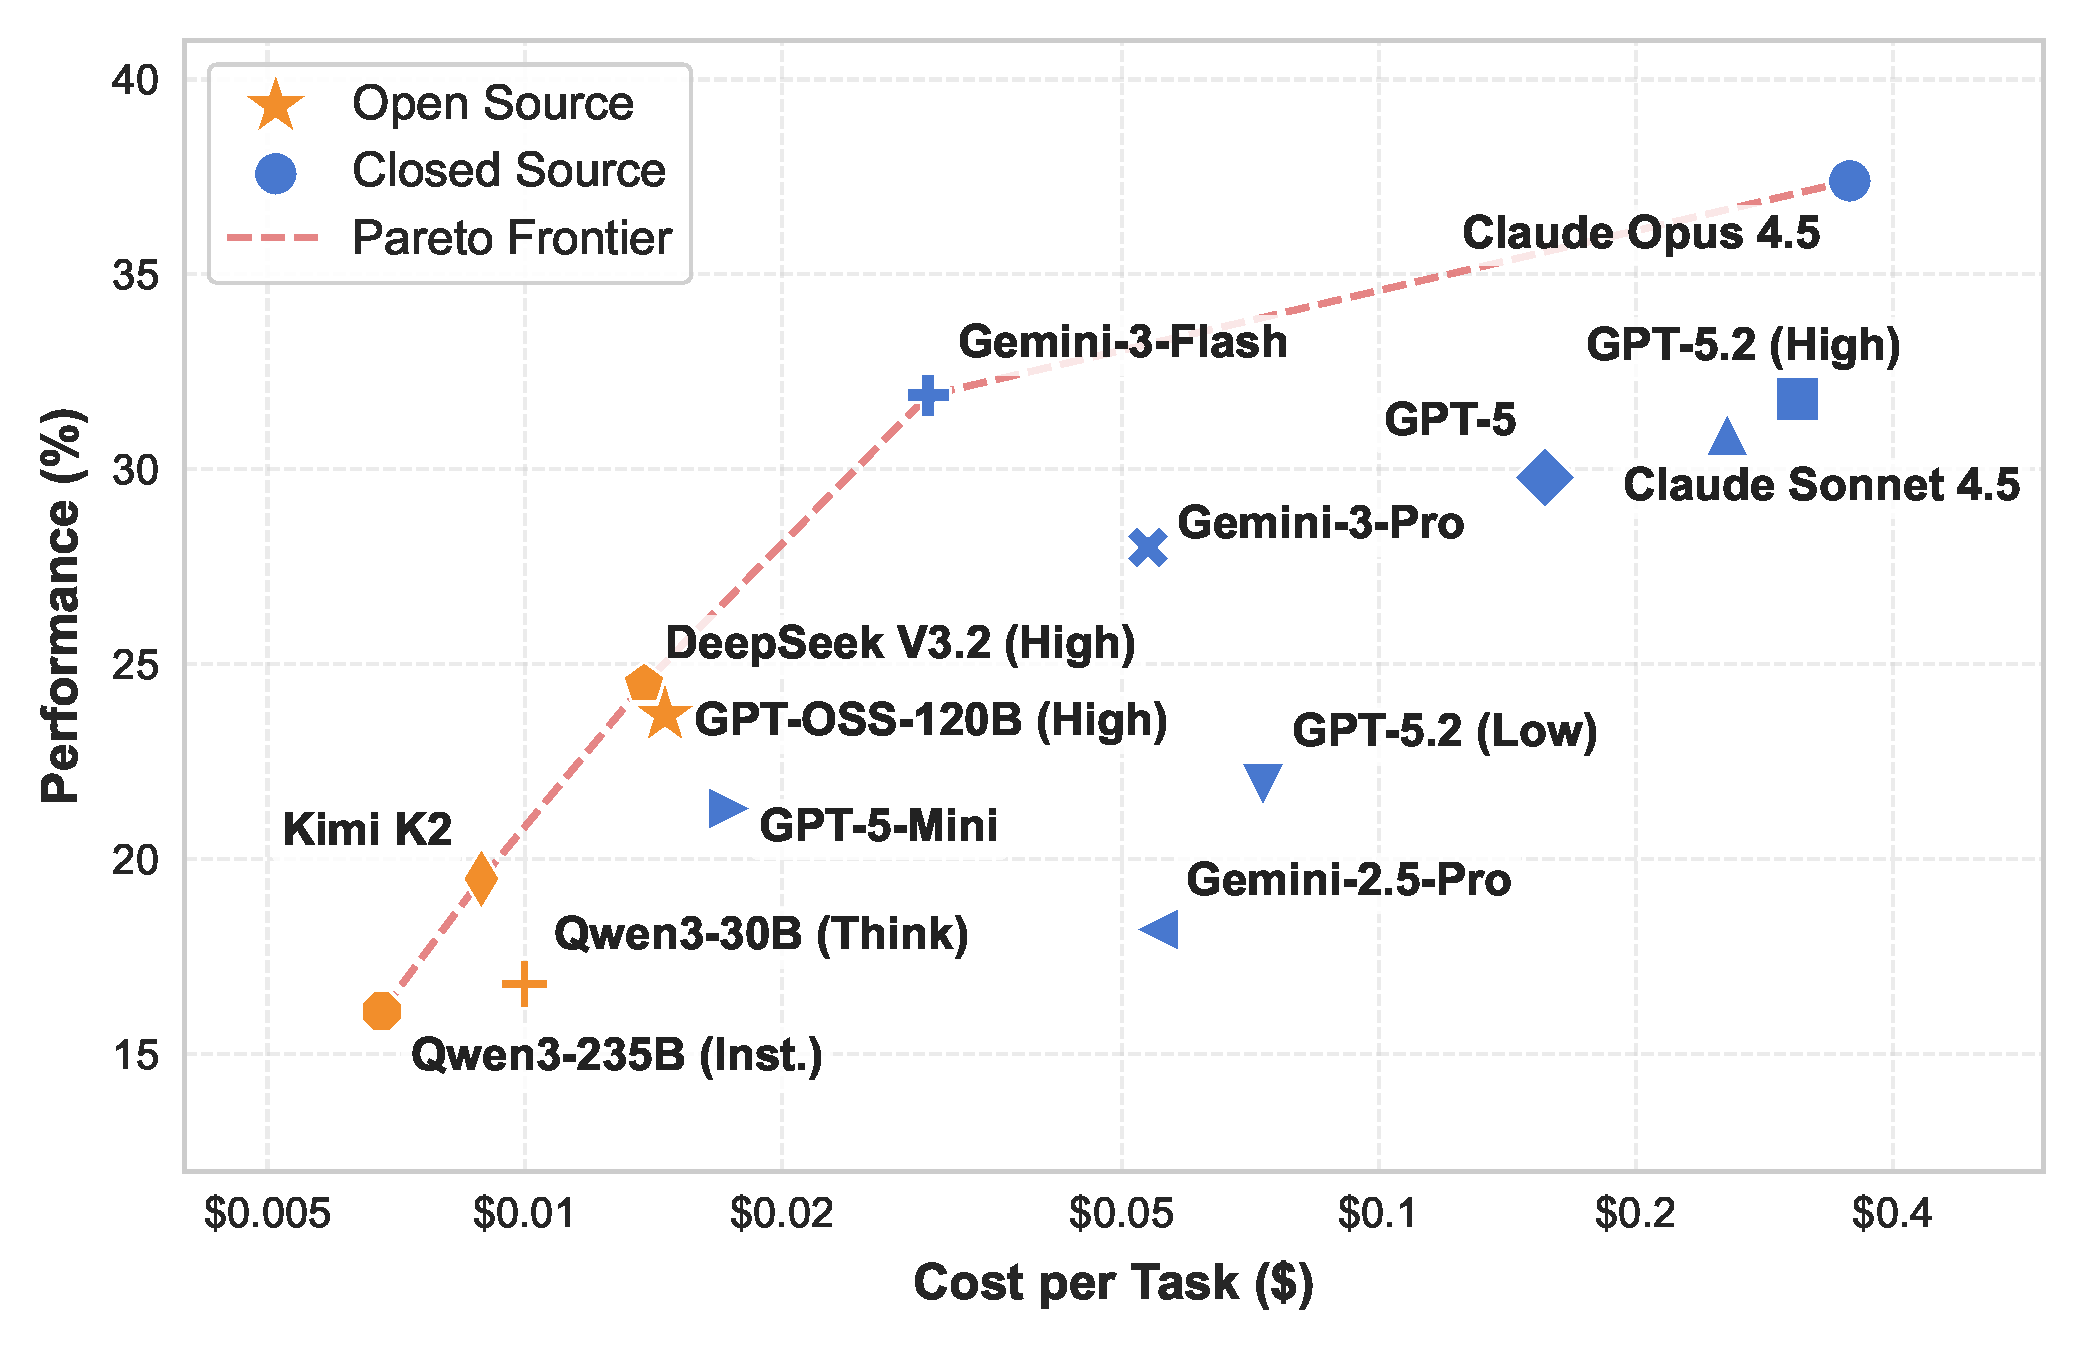
\includegraphics[width=1.0\linewidth]{figures/experiments/cost_vs_perf_new.pdf}
    \caption{\textbf{Performance–cost tradeoff for agentic tool use on \ours{}} We plot task success rate against estimated cost per task for both closed-source and open-source models. Open-source models incur  lower cost but achieve consistently lower success rates. While higher-cost  models offer modest performance gains, they remain far below reliable task completion.}
    \label{fig:cost_vs_preformance}
\end{figure}

\begin{figure*}[t]
 \centering
 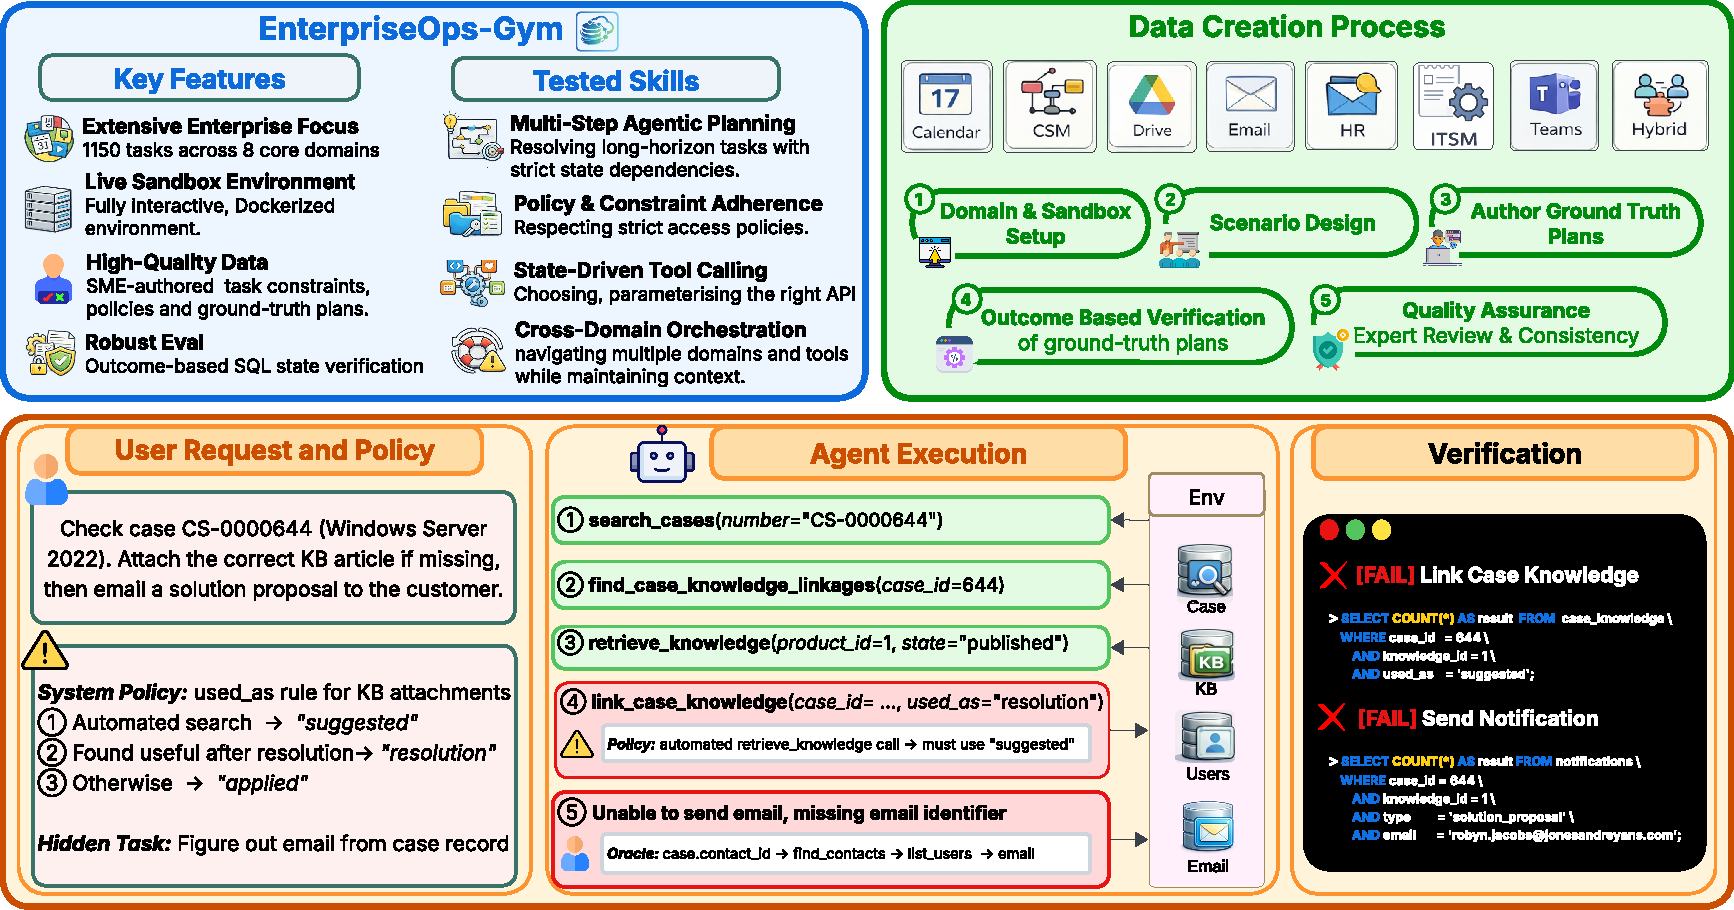
\includegraphics[width=1.0\linewidth]{figures/teaser_final.pdf}

 \caption{\textbf{Overview of \ours{}: A benchmark for stateful agentic planning and tool use.}
(Top-left) \ours{} spans eight enterprise domains and evaluates multi-step agentic planning, policy adherence, state-driven tool calling and cross domain orchestration in a reproducible sandbox. 
(Top-right) Domain experts create sandox and author realistic single- and cross-domain tasks, execute ground-truth trajectories, and write outcome-based verification logic with multi-stage quality assurance along with a human written oracle plan for completing the task. 
(Bottom) Given a task and constraints (as system level policies), agents interact with the environment and execute tools. They are evaluated by final-state verifiers that check goal completion, policy compliance, and side effects. In the above example the agent fails to adhere to system policy for linking case knowledge which mandates setting a parameter to ``suggested'' when a knowledge base is \textit{automatically discovered}. Furthermore, the agent fails to properly send an email notification due to an unresolved identifier for the given case.}


 \label{fig:gym_teaser}
\end{figure*}

\section{Introduction}

LLMs today are most commonly deployed as conversational assistants, answering questions, drafting emails, and summarizing documents \citep{openai2025gpt5, anthropic2025sonnet45}. But a far more consequential capability is rapidly emerging, namely LLMs as \textit{autonomous agents} that act on behalf of users \citep{xu2024theagentcompanybenchmarkingllmagents}. Consider an agent that, from a single instruction, searches the web for real-time inventory data, identifies the best product, and executes the purchase, all without further input. Recent advances in planning and tool use have made the vision of an \textit{AI worker} increasingly plausible: autonomous agents handling professional workflows from software engineering~\citep{jimenez2024swebench} and data analysis \citep{workarena2024} to sales operations and enterprise administration~\citep{huang-etal-2025-crmarena, huang-etal-2025-crmarena-pro}.  Yet to function effectively in real-world professional deployments, such agents must do more than follow instructions. They must (1) maintain state coherently across long sequences of interleaved tool calls, (2) execute multi-step plans spanning dozens of actions, and (3) strictly adhere to the access control policies and procedural rules that govern the workplace.

These requirements are especially relevant within the enterprise domains. Here, agents do not merely retrieve information; they directly modify live databases, trigger downstream workflows, and affect real users. Actions are stateful and often irreversible, errors propagate silently across interconnected systems, and strict organizational policies constrain every step. Figure~\ref{fig:gym_teaser} shows one such example task, where the interplay of the user task and the nuanced system policy constraints demands more than surface-level instruction following. The agent must not only execute a multi-step workflow --- searching a case, retrieving a KB article, and notifying the customer --- but also respect a three-tiered policy governing how KB articles are tagged, and independently resolve a hidden piece of information (the customer's email) by chaining through multiple tools. Equally important, agents must also know when to stop. Blindly attempting a policy-violating task corrupts system state, posing a direct safety risk in production environments.

Despite the urgency of this challenge, existing benchmarks fall short of capturing it. General tool-use evaluations~\citep{li-etal-2023-api, qin2024toolllm, chen2025acebenchwinsmatchpoint} treat tool calls as atomic and stateless, measuring accuracy on short sequences without state dependencies or cross-system coordination. Enterprise-focused benchmarks have emerged~\citep{workarena2024, boisvert2024workarenacompositionalplanningreasoningbased, huang-etal-2025-crmarena, huang-etal-2025-crmarena-pro, jha2025itbenchevaluatingaiagents, vishwakarma2025llmshelpworksandbox} to address challenges in professional environments. While they make important contributions, they are typically confined to a single vendor ecosystem (e.g., Salesforce or ServiceNow alone), with shallow environments of fewer than 25 database tables, under 50 tools, short task horizons, and limited policy constraints governing agent behavior (see \Cref{tab:related_works_comparison}). 

To bridge this gap, we introduce \textbf{\ours{}}, a benchmark designed to evaluate agentic planning within a high-fidelity enterprise simulation. \ours{} spans eight interconnected ecosystems, ranging from general productivity tools like Calendar, Drive, Teams and Email to mission-critical business functions like Human Resource (HR), IT Service Management (ITSM), Customer Service Management (CSM), unified by a Hybrid category demanding coordinated cross-domain execution. The benchmark comprises 1,150 expert-authored tasks across these domains, including 30 infeasible scenarios that test whether agents correctly refuse unsatisfiable requests without leaving side effects on the system. Tasks are verified by hand-written SQL scripts that check goal completion, state integrity, policy compliance, and unintended side effects. \ours{} runs on a fully interactive, containerized environment hosting 164 relational database tables and 512 functional tools, with expert trajectories averaging 9 steps and reaching up to 34. Together, this scale is designed to stress-test the core challenges of enterprise automation: long-horizon planning, cross-system state management, and policy-constrained execution.

Our evaluation of 14 frontier models reveals a significant gap between current agentic capabilities and enterprise requirements. We find that performance is strongly shaped by domain complexity. Models fare best on collaboration tasks, with top models reaching 51--52\% on Email, Teams, and Drive, but drop sharply on policy-governed domains such as ITSM (28.5\%) and cross-domain Hybrid tasks (30.7\%). These are precisely the domains where constraint-aware reasoning is unavoidable. The best overall model, Claude Opus~4.5, achieves only 37.4\%, with open-source models lagging further behind. Infeasibility detection is a critical weak point, with even the best model refusing policy-violating tasks cleanly only 53.9\% of the time. Test-time compute scaling helps but is not a universal remedy, with some workflows plateauing early or showing limited improvements regardless of thinking budget. Importantly, we identify strategic planning and not tool use as the primary bottleneck. Adding distractor tools has negligible impact, while providing human-authored plans improves models by 14--35 percentage points. More complex multi-agent orchestration does not close this gap either; decomposing tasks into subtasks can even regress performance due to strong sequential state dependencies. Together, these results underscore that current agents are not yet ready for autonomous enterprise deployment.

Overall, our contributions are as follows:
\begin{itemize}
    \item We introduce \ours{}, a benchmark of 1,150 expert-curated tasks across eight enterprise domains with outcome-based verification enforcing goal completion, state integrity, policy compliance, and side-effect checks, including 30 infeasible tasks designed to evaluate safe refusal behavior.
    \item We develop a fully interactive, containerized enterprise environment with 164 relational database tables and 512 functional tools, an order of magnitude more complex than prior enterprise benchmarks.
    \item We evaluate 14 frontier models, uncovering and analyzing systematic failure patterns across planning, state management, and policy compliance, and provide actionable insights to build more reliable enterprise agents. We also release \ours{} to the community to advance research in stateful agentic planning and enterprise tool use.
\end{itemize}